%%%%%%%%
%
\documentclass[12pt, a4]{article}
%
\date{}
\usepackage{float}
\usepackage{bibentry}
\usepackage{fancyvrb}
\usepackage{epigraph}
\renewcommand{\epigraphsize}{\footnotesize}
\setlength{\epigraphwidth}{9cm}
\usepackage[dvips]{color}
\usepackage[utf8]{inputenc}
\usepackage[draft]{fixme}
\usepackage{xspace}
\usepackage{colortbl}
\usepackage{ifpdf}
\usepackage[english,italian]{babel}
\usepackage{amsmath}
\usepackage{ntheorem}
\usepackage{hyperref}
\usepackage[numbers,sort&compress]{natbib}
\newcommand{\cchapter}[4]{
\dropchapter{-2cm}
\chapter{#1}
\vskip2cm
\epigraph{#2}{\textit{#3}\\\textit{#4}}
\newpage
}
\usepackage[pdftex]{graphicx}
\newcommand{\HRule}{\rule{\linewidth}{0.5mm}}
%\usepackage{vertbars}
\theoremstyle{definition}
\newtheorem{mydef}{Definition}

%%%%%%%%%%%%%%%%%%%%%%%%%%%%%%%%%%%%%%%%%%%%%%%%%%%%%%%%%%%%%%%%%%%
\begin{document}

\selectlanguage{english}
%
%
%\maketitle                     
\title{Prova}
\begin{titlepage}

\begin{center}


% Upper part of the page

\includegraphics[width=0.25\textwidth]{logo-big}\\[1cm]
\textsc{\LARGE University of Trento}\\[1cm]
\textsc{\Large PAF-FPE: Privacy aware content filtering for future pervasive environments }\\[0.5cm]


% Title
\HRule \\[0.4cm]
{ \huge \bfseries Simluator documentation, vers. 0.1}\\[0.4cm]

\HRule \\[1.5cm]

% Author and supervisor
\begin{minipage}{0.4\textwidth}
\begin{flushleft} \large
\emph{Author:}\\
\textsc{Leonardo Maccari}
\end{flushleft}
\end{minipage}
\begin{minipage}{0.4\textwidth}
\begin{flushright} \large
DISI: Department of Information Engineering and Computer Science 
\end{flushright}
\end{minipage}

\vfill

% Bottom of the page
{\large \today}\\[0.5cm]
{A project financed by: The Trentino programme of research, training and mobility of post-doctoral researchers, incoming Post-docs 2010, grant \#40101857}
\end{center}

\end{titlepage}

\tableofcontents              
\newpage

\section{Introduction}

This simulator is a derivation from Inet 1.99.1 version, it will be probably
updated in the future when the version 2.0 comes out and is intended to perform
mesh/ad-hoc networking simulations using as much as possible realistic
conditions. 
The aim of this project is to study the privacy features of an ad-hoc network
used as a communication base for a social network. This fork of inet provides
the basic blocks to be able to simulate this kind of network with realistic
applications, mobility and channel models. 

Changelog
\begin{itemize}
\item Version 0.1 contains:
\begin{itemize}
\item Musolesi mobility model ported to Omnet with various modifications
\item Raytracing from Omnet by Christian Sommers (obstacles definition) and
Dual Slope pathloss model
\item Obstacle avoidance for LineSegmentsMobility (and consequently for any
other module based on that)
\item AddressGenerator module to have a fresh pool of addresses for the
applications
\item ChatApp application with literature-based statistics and behaviour
\item Initial implementation of firewalling strategies (this will be documented
soon)
\item Tests scenarios for realistic networking
\end{itemize}
\end{itemize} 
\section{Constributed source code}

\subsection{Musolesi Mobility}
This mobility model has been detailed by Musolesi et. al. in various papers, it
is a realistic model derived from social theory of communities, that is, it
generates random traces according to the actions a community of people performs
based on social studies.  The source is not really polished, but the original
code itself was some kind of c-style c++ that should be rewritten from scratch.
I obviously preserved the original LGPL license.

The main idea is the following (even though some details are more complex than this):

\begin{itemize}
\item    divide the space in blocks, x rows and y columns
\item    divide the n nodes in g groups, fill a nxn matrix with 1 where nodes are in the same group and 0 otherwise.
\item    rewire the matrix, that is, with certain probability some links are broken and some new ones are created (so that groups are not disjoint)
\item    assign to each group a block, place the nodes inside that block
\item    now each node ranks the blocks with a weight that is the sum of the non-zero links it has in that block. The highest ranked one is the next target.
\end{itemize}

The ranking of the blocks (calculated by a single node) changes with time, so
nodes in different moments will have different targets. As the paper shows this
mobility model has a high statistical similarity with real traces measured in
various experiments around the world, i.e. the distribution of the contact time
(the time a couple of nodes spend in the same neighborhood (that in my
implementation is approximated with the block they stay in)) and the
inter-contact time (interval between two contacts) is a power-law and not an
exponential as in random way point, that changes the behavior of the network.
The ranking is a deterministic function, so there are various modifications in
order to support periodic reshuffling of the groups or rewiring, without
modifications the nodes all collapse in a single block that behaves like a
magnet. Two modifications are: the assignment of a non-zero rank to all blocks
independently by the nodes that reside in it and then random choice of the block
with probability proportional to the rank, second is presented in a following
paper where the model has been modified introducing a parameter that gives the
probability of “going back home” independently from the other’s position.

In my implementation there are two more differences: the first is that once the
rank has been calculated (with initial non-zero weight)  the target block is
then chosen as a random number with exponential distribution (1/average is
parametrized) this produces a strong bias on the most attractive ones, but adds
some turbolence to the choice. This is much more controlled than uniform choice,
since even if the initial weight is little, the number of blocks may be high and
spread the choice. The second one is that if you insert obstacles into the
scenario the nodes will try to avoid them. This is very basic and it works like
this:
\begin{itemize}
\item Nodes never enter obstacles, so their initial position is never inside an
obstacle and they never chose a target point inside an obstacle
\item If a node realizes that the next step to the chosen waypoint is inside an
obstacle, it choses an intermediate waypoint that is a random point close to the
corner of the obstacle that is on the shortest path to the original waypoint. 
\item When it arrives to the intermediate waypoint it switches the next waypoint
to the original one. Since the intermediate is chosen at random, it may be that
he is going to hit a wall again (and do the procedure again with another random
point. Note that this means he is just wolking a few more meteres, he never goes
around the obstacle over and over) but this saves me from calculating gradients
and doing smarter things.
\end{itemize}

Obstacle avoidance works only if the obstacles are not concave (in this cas you
should do something better than this) and there is enough room between obstacles
so that a random point can be chosen close to a corner of an obstacle with reasonable
probability of not falling into another obstacle. In practice I've tried with
rectangular obstacles spaced at least 10m but you can play with source code.

Note that you could chose a pathological situation, for instance you put an
obstacle that covers an entire block and a nde decides (due to Musolesi's logic)
to go into that block. This obviously doesn't work so you should avoid this. In
the simulator there are counters that check when the simulator is not able to
choose a random point and will raise an error. 

Note that if you run one of the examples with obstacles on Tkenv you will see a
grid corresponding to musolesi blocks (if they are squared, omnet is not able to
show a non-squared grid) and also the obstacles, this helps placing them sanely. 

The most relevant parameter are:
\begin{itemize}
\item    minHostSpeed/maxHostSpeed: speed is chosen randomly in this interval
\item    connectionThreshold: when randomizing the groups give random value to the matrix between 0,1. If the value is higher than this threshold then there is a link (discretized to 1) numberOfRows/numberOfColumns
\item    rewiringProb: when rewiring the matrix, each link value is changed with this probability
\item    rewiringPeriod: rewiring interval
\item    reshufflePeriod: reshuffling interval
\item    numberOfGroups
\item    girvanNewmanOn: this is an alternative way of building the groups, I’ve not been able to make it work from original code…
\item    targetChoice: deterministic/pseudodeterministic/proportional, see the paragraph on ranking
\item    recordStatistics: output some statstics to test the model
\item    drift: the inital weight of a block
\item    expmean: exponential distrbution parameter for pseudodeterminstic
\item    reshufflePositionsOnly: do not reshuffle the groups composition, just change their base block
\item    RWP:  disable group movements, just a random way point. This has been added just to perform statistical comparisons numHosts
\item    hcmm: Boldrini modifcation, this is the probability of going back home
\end{itemize}


To better understand how the mobility model works go to
\href{http://pervacy.eu/?p=78}{this link} where you have some videos I've
realized to show the mobility and the dependency of the statistical properties
by the parameters.

\subsection{Address Generator}
This module is an address generator that the applications can use to choose
the destination of the sessions they open. The need for this is that each
application takes care of choosing where to send the next packet, but it does
this quite simply, whether you specify it on configuration or, some, take a
random() keyword meaning anyone. In wireless ad-hoc simulations this does not
work since the network is often disconnected and you may not want your
application to send packets to somebody that is not reachable now (this
obviously applies to proactive routing). So the module uses the current routing
table to give a list of address that are effectively reachable and returns the
list to the application that is requesting them. You can do also more simple
things like fixed list or random addresses.  The main configuration items are:

\begin{itemize}
\item    string generatorMode = default(“RoutingTable”):  The way addressess are
gathered, this can be (you can mix 1 and 3):
\begin{enumerate}
\item        RoutingTable: get them from your routing table (useful in ad-hoc networks)
\item        FixedList: get them from the configuration
\item        NodeType: specify a node type and get any of them
\end{enumerate}
\item    int listSize = default(-1):  size of the list to be returned.
\item    string addressList = default(“”): needed for FixedList mode, may be “random(host)” where host is the nodetype
\item    string nodeType = default(“”); needed for NodeType mode
\item    string routingTablePath = default(“”); it it is unset, the default is host[].routingTable
\item    int waitTime @unit(s) = default(1s):  when using routingTable mode do not start at time==0 but wait an amount of time, this is useful when routing tables take some time to be filled and keepSetConsistent is used
\item    bool keepSetConsistent = default(false): try to keep time consistency of the list among updates (not just random IP taken by routes, safeguard the ones already present in the list at previous iteration)
\item    bool keepSetBalanced = default(false); try to keep topology consistency of the list among updates. In group mobility models the keepSetConsistent will probably produce sets with a lot of one-hop nodes since they are always reachable. This tries to proportionally spread the target set over the possible hopcount in the network.
\item    int updateTime @unit(s) = default(1s): The time interval to refresh the address pool. Keep this high if possible, since refreshing the pool can be expensive with large routing tables.
\end{itemize}

The last two options prove to be useful when you want to limit the set of
possible target nodes. For instance, you want your application to talk to only a
subset of n nodes over the N present in the network. Since the routing table changes with time (if
you have mobility) every time you ask for a set of target address you will
receive  n random addresses over N. You may instead want to keep it as
consistent as you can (that is after a certain subset has been chosen, the next
time keep the in the set the nodes that were in the previous choice and are
still reachable). 

With certain mobility models, keeping the target set consistent is not a good
idea, for instance with cluster-based models such as Musolesi’s model your 1-hop
neighbor set does not changes often. If you keep it consistent you will
basically talk only with one-hop neighbors. The keepSetBalanced instead gets the
n addresses taking into account the distance in hop (well, in the metric value)
and tries to give you a set that is uniformly distributed over the possible
metric value.

\subsection{Dual Slope}

Dual Slope introduces one breakpoint distance at which the decay coefficient
changes, the rationale is to simulates situations in which the two communicating
nodes are in LOS up to a certain distance and NLOS after that distance (or other
effects that influence the pathloss). You can choose the two coefficients and
the distance using the configuration parameters. There is one more parameter
that is used to avoid producing a hard step at the breakpoint distance, if you
enable it a smoothing factor is used. Configurations are quite straightfoward. 
See \href{http://pervacy.eu/?p=65}{this link} for graphics.

\section{Scenario Documentation}

The scenarios are included in order to give a starting point for anyone that
wants to simulate an ad-hoc or mesh network without wasting too much time to
set-up a realistic environment. The scenarios are divided according to various
criterias:
\begin{itemize}
\item Ad-hoc/Mesh: the first case is a completely ad-hoc network, in the other
case there is a mesh network with fixed nodes (and more powerful radio)
distributed with a grid topology plus some ad-hoc nodes roaming
\item Little/Middle/Big/Fat: the size of the area and number of nodes. Fat
stands for Middle area with more nodes into it.
\item SlowMobility/FastMobility: there is a difference in the average speed of
nodes, in the mobility update time, in the frequency of the generation of
packets from the applications and in the duration of the simulation.
Basically fast simulations are used to test the changes you implement and slow
ones are imagined to get real results
\item Obstacles: in presence of obstacles the grid may be substituted with a
wiser placement of the mesh nodes, as in the figure below, which resambles a
simplified topology of the area around the DISI department.
\end{itemize}

The scenarios are defined in various .ini files, one for topology and mobility,
one for traffic and another one to sum up everything. 

For each scenario in the anf/ folder you can find some evaluation parameters,
they include the average arrival rate of the echo applications (there are 25
available ports on each mobile node pinged randomly by udpApp[26]), average
routing table size, average hopcount, average chat session run. See appendix for
example images. 


\begin{figure}
\begin{center}
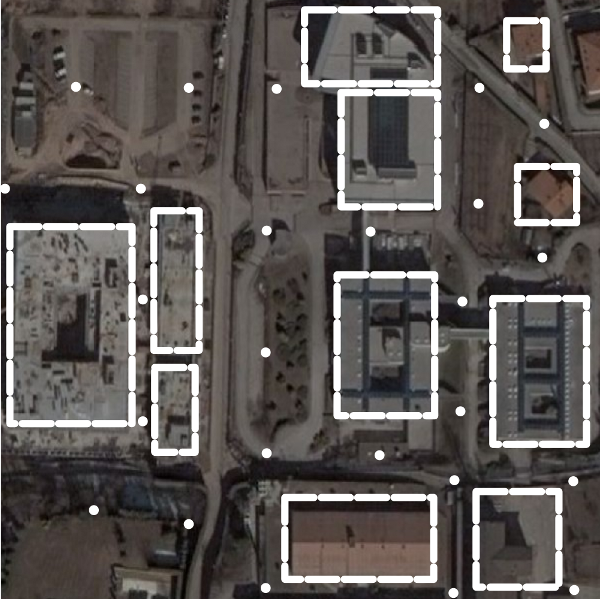
\includegraphics{povo600}
\end{center}
\end{figure}
\section{OLSR and firewalling}

Most of the modifications deal with OLSR and firewall implementation, which I
will document in the future. I didn't try the scenarios with other routing
algorithms.

\appendix
\section{Scenario results}

All the \emph{Slow} scenarios guarantee a delivery of UDP packets between 90\%
and 97\% but the big and fat ones, which go around 85\%. To behave better, they
would need some more attention and some more optimization, starting with power
control and OLSR\_ETX (ETX metric)

\begin{figure}
\begin{center}
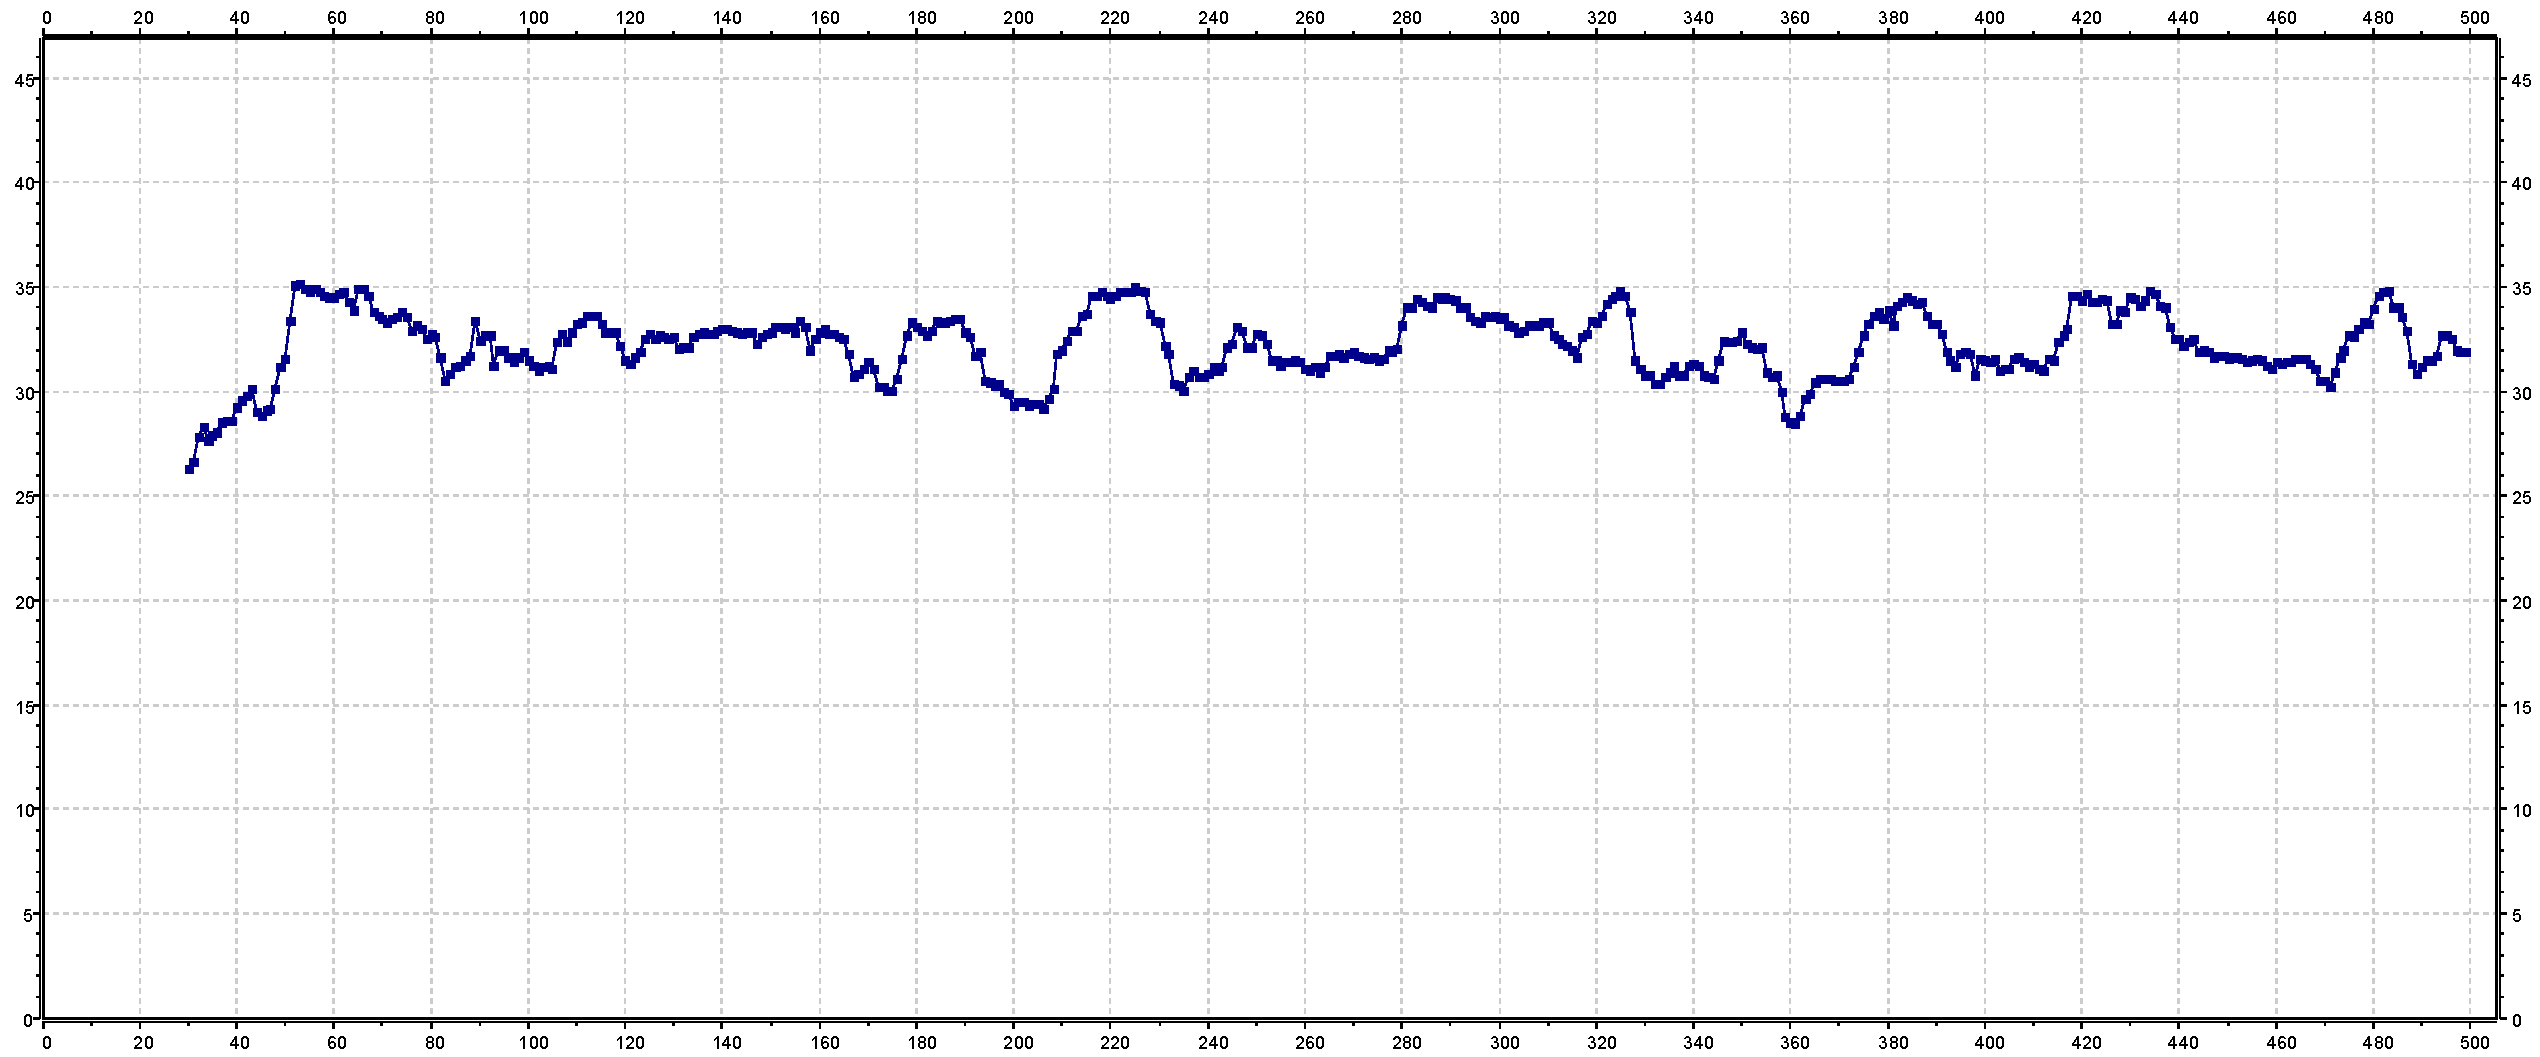
\includegraphics[scale=0.35, angle=90]{images/AdHocLittleAreaFastSquaredRouting}
\caption{Routing table size averaged for all the nodes, reported as a vector. To have an always
connected ad-hoc network (without power control) the hopcount would be too low
and the capacity would fall down. I chose to have an almost always-connected
network and use addressGenerator to talk only to nodes that are effectively
reachable. Nevertheless we have some loss}
\end{center}
\end{figure}

\begin{figure}
\begin{center}
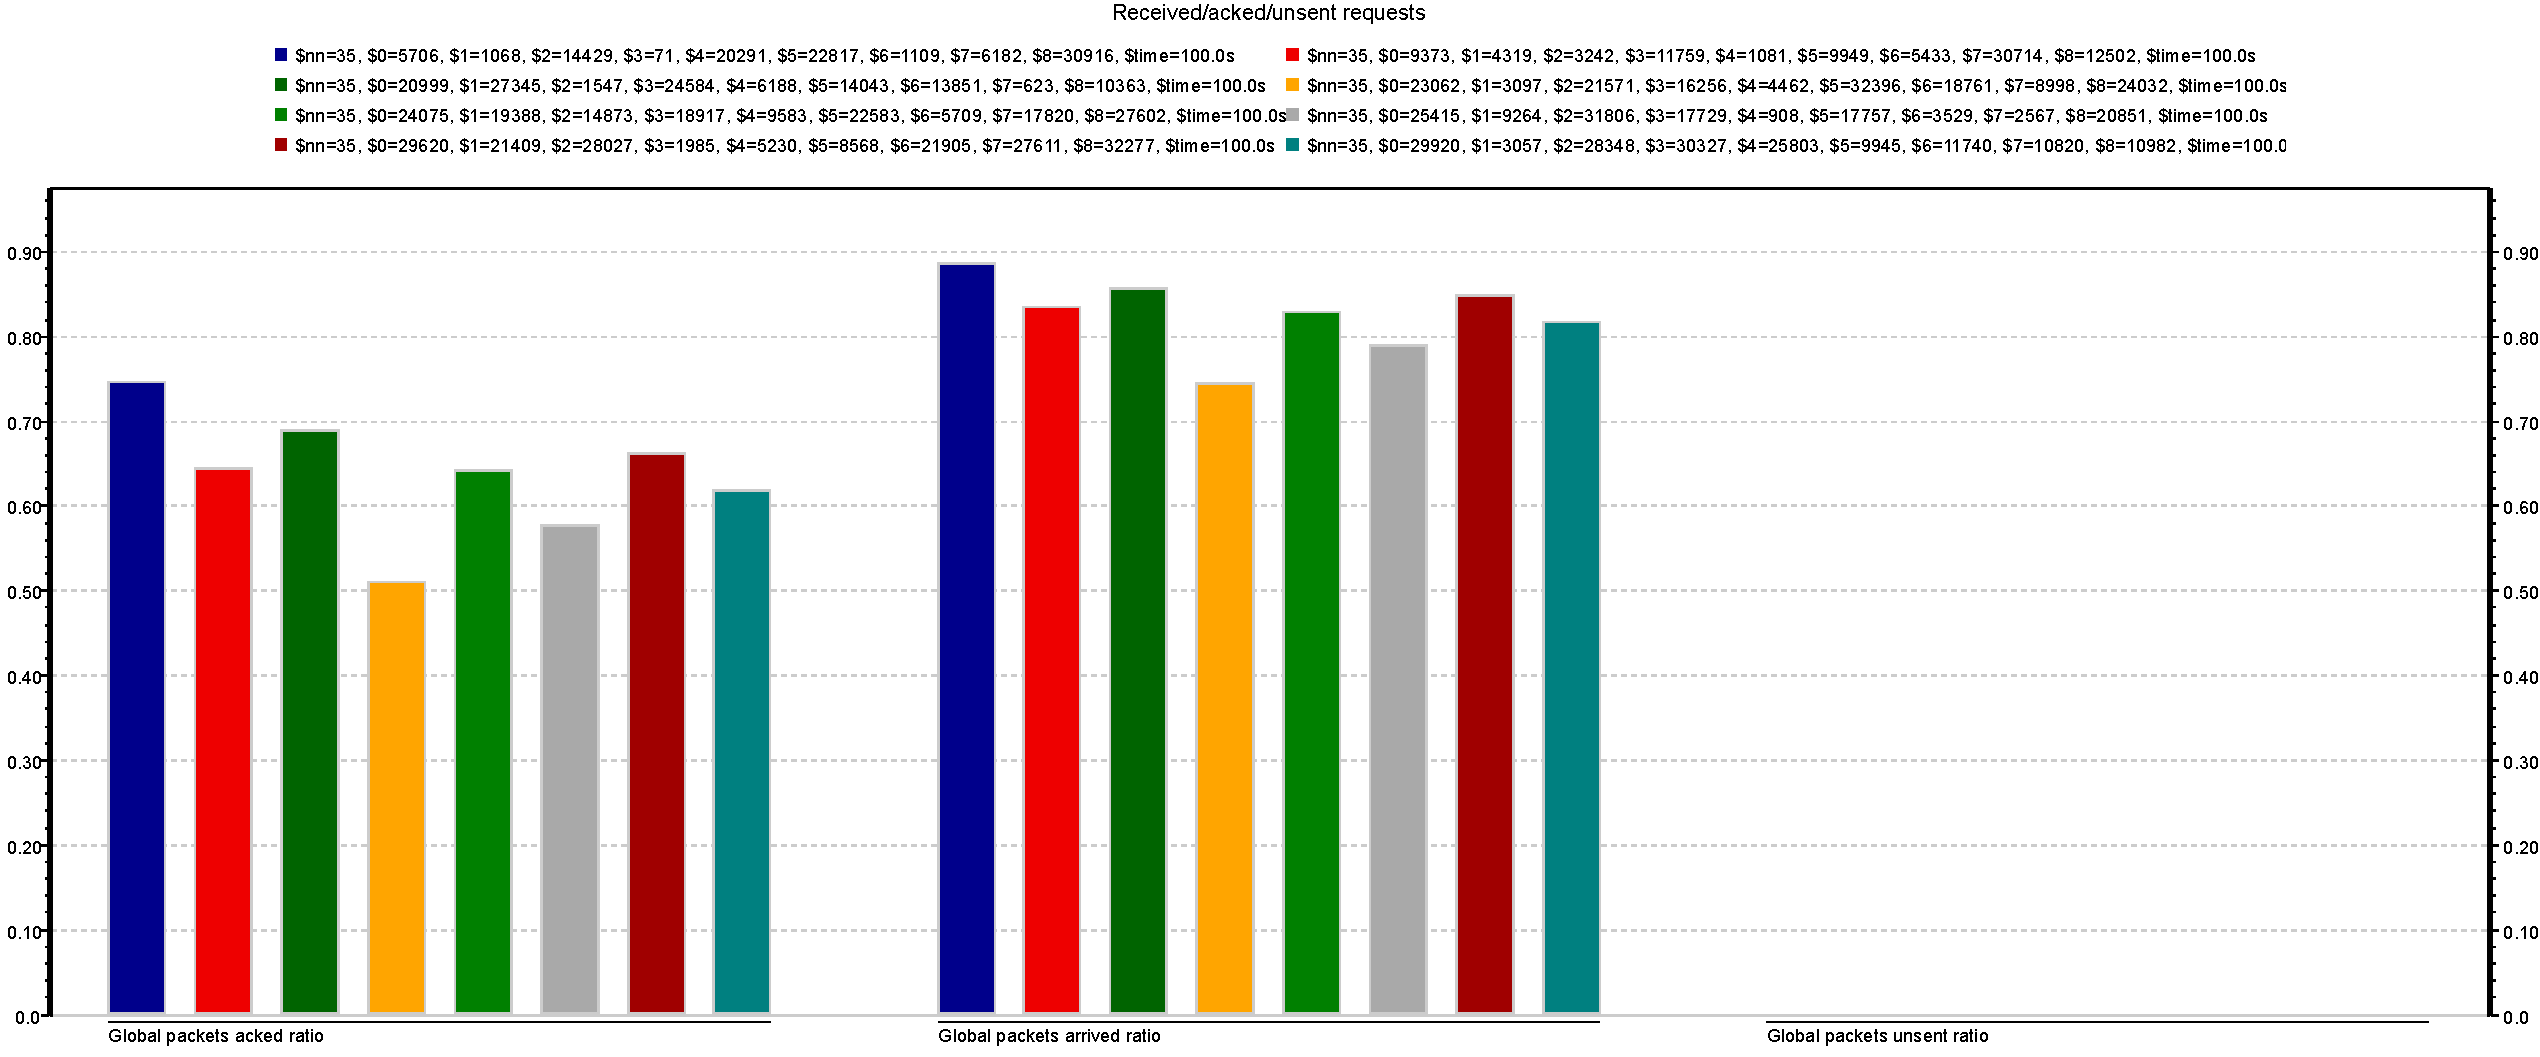
\includegraphics[scale=0.35, angle=90]{images/AdHocLittleAreaFastSquared}
\caption{The ratio of received packets, of acket packets and unsent packets.
Unsent are counted when there are no available addresses to be used (the node is
isolated, may happen rarely)}
\end{center}
\end{figure}


\begin{figure}
\begin{center}
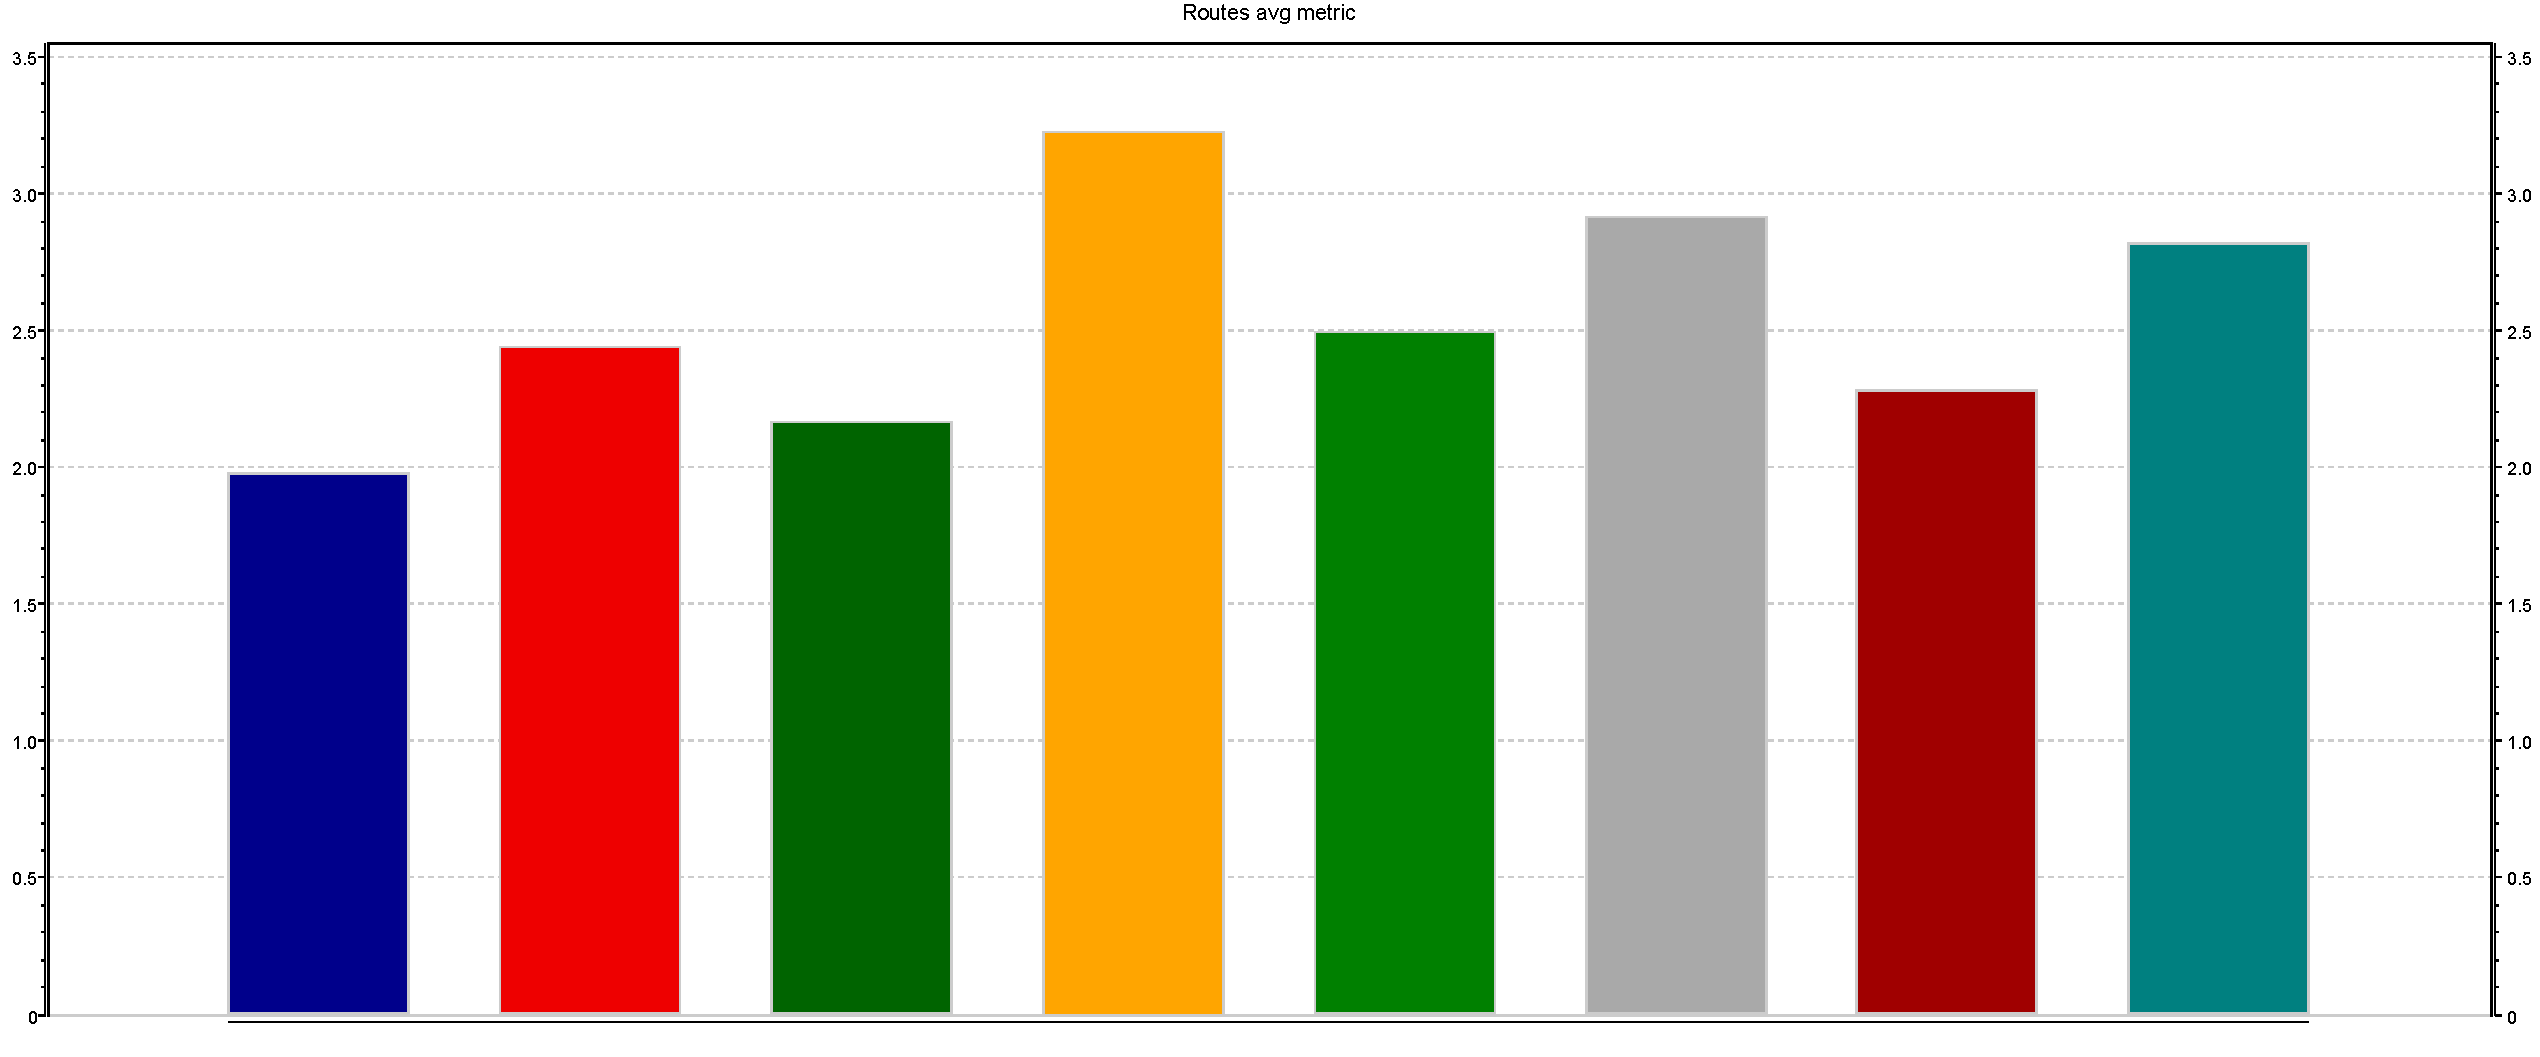
\includegraphics[scale=0.35, angle=90]{images/AdHocLittleAreaFastSquaredHc}
\caption{This is the average hopcount measured from the metric field in the
routing table}
\end{center}
\end{figure}

\begin{figure}
\begin{center}
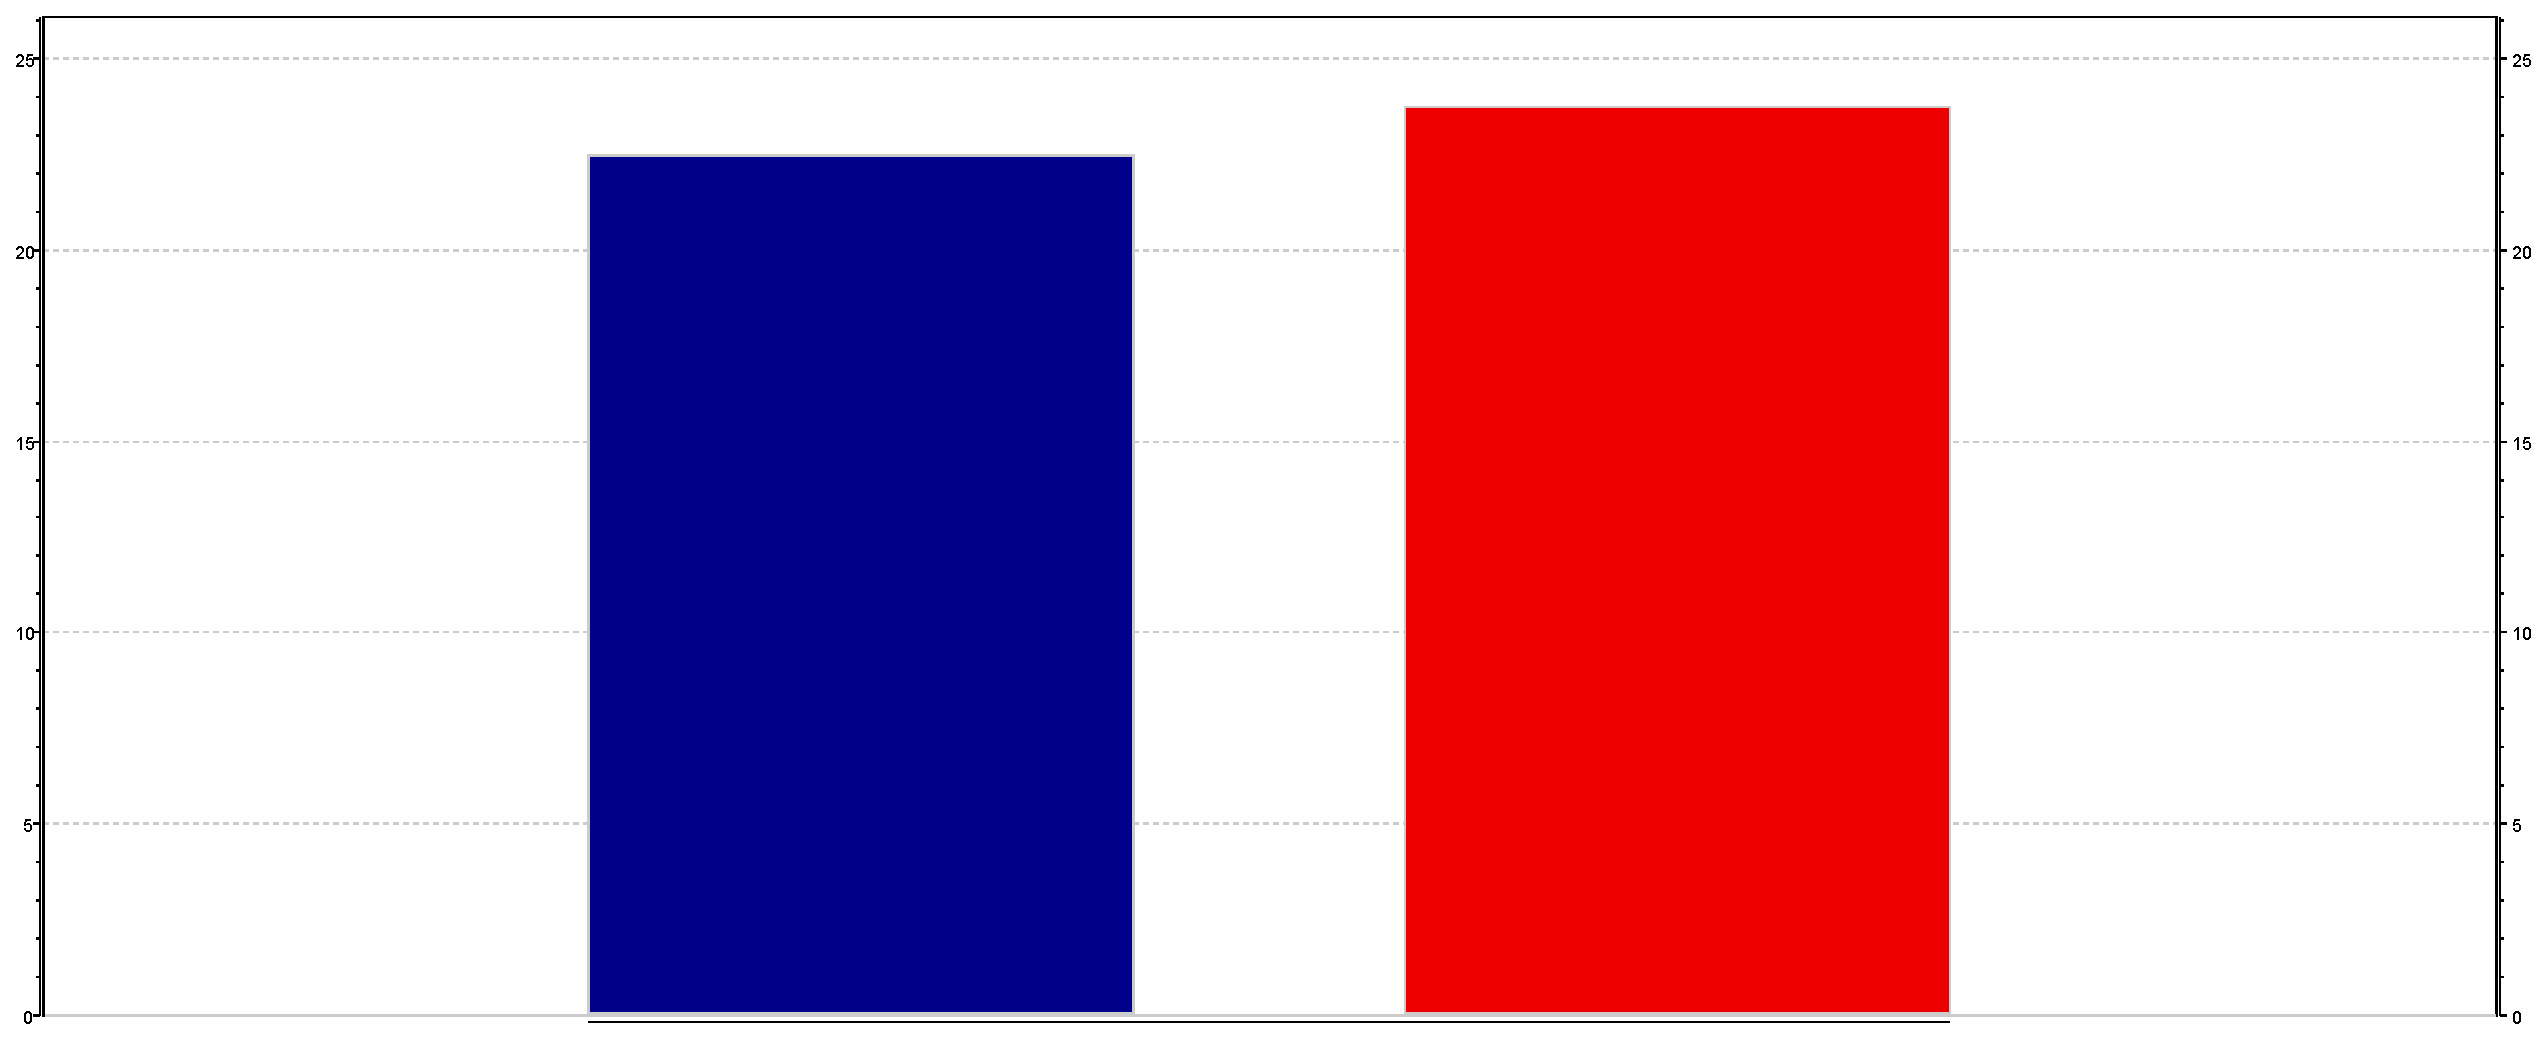
\includegraphics[scale=0.35]{images/AdHocLittleAreaFastSquaredChat}
\caption{Chat sessions started and received from node 0}
\end{center}
\end{figure}



\newpage
\section{License}
All the documentation including, pdf, source .tex files and images are
copyright by Leonardo Maccari and released using a Creative Commons
Attribution-NonCommercial-ShareAlike 3.0 Unported License license.

Which means that you are free:

\begin{itemize}
\item to Share — to copy, distribute and transmit the work
\item to Remix — to adapt the work
\end{itemize}

Under the following conditions:

\begin{itemize}
 \item   Attribution — You must attribute the work in the manner specified by the author or licensor (but not in any way that suggests that they endorse you or your use of the work).

 \item   Noncommercial — You may not use this work for commercial purposes.

 \item   Share Alike — If you alter, transform, or build upon this work, you may distribute the resulting work only under the same or similar license to this one.
\end{itemize}

With the understanding that:

\begin{itemize}
 \item   Waiver — Any of the above conditions can be waived if you get permission from the copyright holder.
 \item   Public Domain — Where the work or any of its elements is in the public domain under applicable law, that status is in no way affected by the license.
 \item   Other Rights — In no way are any of the following rights affected by the license:
        Your fair dealing or fair use rights, or other applicable copyright exceptions and limitations;
        The author's moral rights;
        Rights other persons may have either in the work itself or in how the work is used, such as publicity or privacy rights.
 \item   Notice — For any reuse or distribution, you must make clear to others the license terms of this work. The best way to do this is with a link to this web page.

\end{itemize}

\bibliographystyle{IEEEtran}
\bibliography{bibliography}
%
\end{document}
